%\documentclass[fleqn,10pt]{wlscirep}
% switch bib style for arxiv
\documentclass[fleqn,10pt]{scipy}

% Packages
\usepackage[super]{nth}
\usepackage{rotating}
\usepackage{makecell}
\usepackage{pifont}
\usepackage{amsfonts}
\usepackage{amsmath}
\usepackage{float}
\usepackage{pgfplots}

\pgfplotsset{compat=newest}
\usepackage{listings, textcomp}

\lstset{ %
  basicstyle=\ttfamily\footnotesize,  % size of fonts used for the code
  breaklines=true,   % automatic line breaking only at whitespace
  captionpos=b,   % sets the caption-position to bottom
  commentstyle=\color{gray},  % comment style
  keywordstyle=\color{blue},  % keyword style
  stringstyle=\color{red},  % string literal style
  upquote=true  %straight single quotes (requires textcomp)
}

% New Commands
\newcommand{\cmark}{\ding{51}}%
\newcommand{\xmark}{\ding{55}}%
\newcommand{\code}[1]{\texttt{#1}}

\title{SciPy 1.0---Fundamental Algorithms for Scientific Computing in Python}

\author[1]{Pauli Virtanen}
\author[2,*]{Ralf Gommers}
\author[3,4]{Tyler Reddy}
\author[5]{Anne Archibald}
\author[6]{Andrew Nelson}
\author[7]{Charles Harris}
\author[8]{CJ Carey}
\author[9]{Denis Laxalde}
\author[10]{Eric Larson}
\author[11]{Eric Moore}
\author[12]{Eric Quintero}
\author[13]{Evgeni Burovski}
\author[14]{Jaime Fernández del Río}
\author[15]{Josef Perktold}
\author[16]{Josh Wilson}
\author[17]{Matthew Brett}
\author[18]{Nikolay Mayorov}
\author[19]{Warren Weckesser}
\author[20]{Matt Haberland}
\author[21]{Scott Sievert}
\author[22]{Yu Feng}
\author[23]{Antonio Horta Ribeiro}

\affil[1]{Affiliation, department, city, postcode, country}
\affil[2]{Affiliation, department, city, postcode, country}
\affil[2]{Affiliation, department, city, postcode, country}
\affil[3]{UC Berkeley Institute for Data Science,
          Berkeley, CA, 94720, USA}
\affil[4]{Los Alamos National Laboratory,
	  Theoretical Division 6,
          Los Alamos, NM, 87545, USA}
\affil[5]{Affiliation, department, city, postcode, country}
\affil[6]{Affiliation, department, city, postcode, country}
\affil[7]{Affiliation, department, city, postcode, country}
\affil[8]{Affiliation, department, city, postcode, country}
\affil[9]{Affiliation, department, city, postcode, country}
\affil[10]{Affiliation, department, city, postcode, country}
\affil[11]{Affiliation, department, city, postcode, country}
\affil[12]{Affiliation, department, city, postcode, country}
\affil[13]{Affiliation, department, city, postcode, country}
\affil[14]{Affiliation, department, city, postcode, country}
\affil[15]{Affiliation, department, city, postcode, country}
\affil[16]{Affiliation, department, city, postcode, country}
\affil[17]{Affiliation, department, city, postcode, country}
\affil[18]{Affiliation, department, city, postcode, country}
\affil[19]{Affiliation, department, city, postcode, country}
\affil[20]{Affiliation, department, city, postcode, country}
\affil[21]{Affiliation, department, city, postcode, country}
\affil[22]{Affiliation, department, city, postcode, country}
\affil[23]{Affiliation, department, city, postcode, country}

\affil[*]{ralf.gommers@gmail.com}

\keywords{Scientific computing, Python, Mathematics}

% NOTE: some usage stats below are from https://libraries.io/pypi/scipy
% as well as github metrics; normally one doesn't put citations directly
% in abstract though (depends on field / journal)
\begin{abstract}
SciPy is an open source scientific computing library for the Python programming language.
SciPy 1.0 was released in late 2017, about 16 years after the original
version 0.1 release. SciPy
has become a \emph{de facto} standard for leveraging scientific algorithms
in the Python programming language, with more than 600
unique code contributors, millions of downloads per year, 161 dependent
packages, and 28700 dependent respositories.
The library includes functionality spanning clustering, Fourier transforms,
integration, interpolation, file I/O, linear algebra, image processing,
orthogonal distance regression, minimization algorithms, signal processing,
sparse matrix handling, computational geometry, and statistics. In this
work, we provide an overview of the capabilities and development practices of the
SciPy library and highlight some recent technical developments.
\end{abstract}
\begin{document}

\flushbottom
\maketitle
\thispagestyle{empty}

\section*{Introduction}

\textit{The Introduction section expands on the background of the work (some overlap with the Abstract is acceptable). The introduction should not include subheadings.}

\section*{Background}

Python ... late 1980s



An matrix / n-dimensional array object ...
matrix.py, numeric, numarray, numpy

Paul Dubois

Travis O

Pearu

- 
Gary Strangman

%https://mail.python.org/pipermail/scipy-dev/2001-November/000088.html
%

Eric and Travis V

\subsection*{SciPy Begins}

-  Jun 10, 2001
Travis N. Vaught announced scipy-dev mailing list

- Aug 20, 2001
Eric Jones announced 



IPython 2001 first release

Matplotlib 2003 first release

\begin{figure}
\begin{verbatim}
SciPy is an open source package that builds on the strengths of Python and
Numeric providing a wide range of fast scientific and numeric functionality.
SciPy's current module set includes the following:

    Special Functions (Bessel, hanker, Airy, etc.)
    Signal/Image Processing
    2D Plotting capabilities
    Integration
    ODE solvers
    Optimization (simplex, BFGS, Netwon-CG, etc.)
    Genetic Algorithms
    Numeric -> C++ expression compiler
    Parallel programming tools
    Splines and Interpolation
    And other stuff.
\end{verbatim}
\caption{Excerpt from first release announcement.}
\end{figure}


\subsection*{Conferences}

%https://mail.python.org/pipermail/scipy-dev/2002-June/001007.html

SciPy

US, India, Europe

SIAM CSE

PyData

everywhere...

\cite{siamcse09}

%https://archive.siam.org/news/news.php?id=1595

 

\subsection*{Publications}

CiSE 2007 special issue

CiSE 2011 special issue


\cite{dubois2007guest}
\cite{oliphant2007python}
\cite{perez2007ipython}
\cite{hunter2007matplotlib}
\cite{vanderwalt2008scipy}
\cite{peterson2009f2py}
\cite{millman2011python}
\cite{perez2011python}
\cite{vanderwalt2011numpy}
\cite{behnel2011cython}
\cite{pedregosa2011scikit}
\cite{vanderwalt2014scikit}
\cite{millman2014developing}
\cite{meurer2017sympy}

\subsection*{SciKits}

% stefan, gael, david, jarrod, 


website http://scikits.appspot.com/

statsmodels

scikit-image

scikit-learn



\subsection*{Release History}


ANN: SciPy 0.10 -- Scientific Computing with Python

\begin{figure}
\begin{verbatim}
    2001: first SciPy release
    2005: transition to NumPy
    2007: creation of scikits
    2008: spatial module and first Cython code added
    2010: move to a 6-monthly release cycle
    2011: development moves to GitHub
    2011: Python 3 support
    2012: add a sparse graph module and unified optimization interface
    2012: remove of maxentropy
    2013: continuous integration with TravisCI
    2015: adding Cython interface for BLAS/LAPACK and a benchmark suite
    2017: add a unified C API with LowLevelCallable; remove weave
    2017: SciPy 1.0 release
\end{verbatim}
\caption{Timeline}
\end{figure}

\subsection*{Project goals and scope}

\subsection*{Current status (maturity, users)}


\section*{Architecture and implementation choices}

\subsection*{Submodule organisation}
\input{subpackages}

\subsection*{Common infrastructure}

\subsection*{Language choices}
Python, Cython, Fortran, C and C++ are the programming languages
used to implement scientific algorithms in the SciPy library. An analysis
of our code base using the \texttt{linguist} library provides a detailed
breakdown as \% composition by programming language in SciPy
(Figure~\ref{fig:linguist}).

    \begin{figure}[H]
        \centering

        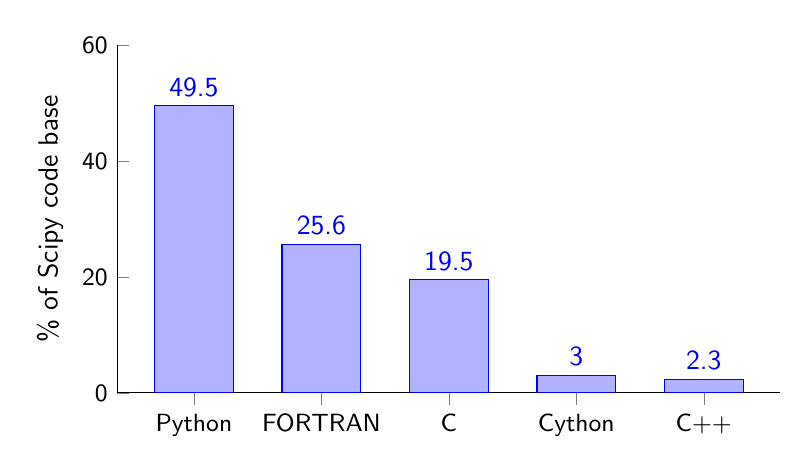
\begin{tikzpicture}[font=\sffamily]
        \begin{axis}[height=6cm, width=10cm,
        ybar, ymax=60, ymin=0,bar width=1cm,
        ylabel={\% of Scipy code base},
        ytick={0,20,...,60},
        axis lines*=left,
        axis y line shift=0pt,
        enlarge x limits=0.15,
        symbolic x coords={py,f,c,cy,cpp},
        xticklabels={Python,FORTRAN,C,Cython,C++},
        ticklabel style={align=center,font=\sffamily\small,
        /pgf/number format/assume math mode=true},
        xtick=data,
        nodes near coords,
        nodes near coords style={/pgf/number format/assume math mode=true}
        ]
        \addplot coordinates {(py,49.5) (f,25.6) (c,19.5) (cy, 3.0) (cpp,2.3)};
        \end{axis}
        \end{tikzpicture}
        \caption{The breakdown of programming languages used in the
	         SciPy library determined using the linguist library.
		 Small ($<0.5 \%$) amounts of TeX, Matlab, Shell,
		 and Makefile are excluded for clarity and mostly
		 provide supporting roles in tests, building, and
		 documentation.}
        \label{fig:linguist}
    \end{figure}

For implementing new functionality, we have a clear order of language preference.
First Python, if performance is not an issue. If it is, then in order of
preference: Cython, C, C++, Fortran. The main motivation for this is 
maintainability: Cython has the highest abstraction level and most 
Python developers will understand it. C is also widely known,
and easier to deal with for the core development team
than C++ and especially Fortran.

While it is not surprising that Python is heavily used in SciPy, the
usage distribution of the other languages warrants some discussion. Fortran
is an extremely well-established scientific programming language, both
for historical reasons and because of its continued excellent
performance\cite{Koelbel:1993:HPF:562354}. We
wrap the FFTPACK Fortran library for performing Fourier
transforms\cite{SWARZTRAUBER198445, SWARZTRAUBER198251} since
this library has been a standard in the field for 33 years and has a license
that is compatible with our own. Likewise, we wrap the Fortran source
for ODEPACK\cite{citeulike:2644528} as it has been  trusted for the initial 
value problem for ordinary differential equation systems for 30 years. For
similar reasons we also wrap the Fortran libraries QUADPACK\cite{1983qspa.book.....P} (for numerical
integration of one-dimensional functions), FITPACK\cite{Dierckx:1993:CSF:151103} (curve-fitting /
interpolation), ODRPACK\cite{ODRPACK_Boggs} (orthogonal distance regression),
MINPACK\cite{osti_6997568} (minimization of linear and nonlinear equations),
ARPACK\cite{leh:sor:yan96} (solving large scale eigenvalue problems), 
ALGORITHM 644\cite{Amos:1986:APP:7921.214331} (handling Bessel Functions), and 
CDFLIB\cite{CDFLIB_site} (evaluation of cumulative density functions).

Rounding out the top three languages in SciPy is C, which is also extremely
well-established over several decades\cite{Kernighan:1988:CPL:576122} of
scientific computing. Alongside its objected-oriented relative C++, C
can be leveraged in Python after being exposed using the Cython
language. Cython has been described as a creole language that mixes
the best parts of Python and lower-level C / C++
paradigms\cite{behnel2011cython}. We thus often use Cython as a glue
between well-established low-level scientific computing libraries and
the Python interface offered by SciPy. We also use Cython to enable
performance enhancements in Python code, especially for cases where heavily
used inner loops benefit from a compiled code with static typing. Some of the C
libraries that we wrap in SciPy include trlib\cite{doi:10.1080/10556788.2018.1449842} 
(iterative solving of the trust region problem), SuperLU\cite{li05,superlu_ug99} (solution of
large, sparse, nonsymmetric systems of linear equations),
Qhull\cite{Barber:1996:QAC:235815.235821} (computational
geometry), and Cephes\cite{cephes_netlib} (mathematics algorithms). 

Therefore, the relative abundance of different programming languages
in the SciPy library results from a combination of the usage of powerful performance
enhancing languages that interact well with Python (i.e., Cython), and
the usage of languages (and their libraries) that have proven reliable
and performant over many decades. The position that SciPy occupies
near the foundation of the scientific Python ecosystem is such that
adoption of new languages or major dependencies is generally unlikely--our
choices are strongly driven by long-term stability. GPU acceleration,
new transpiling libraries, and the latest JIT compilation approaches
(i.e., Numba\cite{Lam:2015:NLP:2833157.2833162}) are very powerful, but currently fall outside the remit
of the main SciPy library. That said, we have recently increased our
efforts to support compatibility with some of these options, and having
our full test suite pass with the PyPy JIT compiler\cite{Bolz:2009:TMP:1565824.1565827}
is now a requirement in our development workflow.

\subsection*{API and ABI evolution}
In general, we encourage changes that improve clarity in the API of the library,
but strongly discourage breaking backwards compatibility, given our position near
the base of the scientific Python computing stack.


\section*{Key technical improvements}

Here we describe key technical improvements made in the last three years.

\subsection*{Data structures}
\textbf{cKDTree}
\input{ckdtree}
\textbf{Sparse matrices}

\subsection*{Unified bindings to compiled code}
\subsubsection*{LowLevelCallable}
As of SciPy version 0.19, it is possible for users to wrap low-level
functions in a \texttt{scipy.LowLevelCallable()} object that reduces
the overhead for calling compiled C functions directly from Python.
Supported low-level functions include \texttt{PyCapsule} objects,
ctypes function pointers, and cffi function pointers. The low level
function signature must be consistent with the expectations of the
routine it is passed to. For example, the documentation for
\texttt{scipy.ndimage.generic\_filter} defines two acceptable C callback
function signatures that may be used to produce functions that operate
on each element of image data with low overhead. The C code may be
generated using numba or Cython, for example, as long as the function
call signature matches the specifications. Furthermore, it is even
possible to generate a low-level callback function automatically
from a Cython module using \texttt{scipy.LowLevelCallable.from\_cython}.

\subsection*{Cython bindings for BLAS, LAPACK and special}

\subsection*{Numerical optimization}
\input{scipy-optimize}


\subsection*{Statistical distributions}

%%%%%%%%%%%%%%%%%%%%%%%%%%%%%
\subsection*{Polynomial interpolators}
\input{poly}

\subsection*{Test and benchmark suite}

    \subsubsection*{Benchmark suite}

    The airspeed velocity (asv) library enables benchmarking Python packages over their lifetimes, and the performance of the SciPy
    code base was monitored with asv starting in February of 2015 (PR \#4501). In addition to ensuring that unit tests are passing (see above),
    confirming that performance generally remains constant or improves over the commit hash history of the project allows us to objectively
    measure that our code base is improving, to empower scientific applications.

    Consider the asv benchmark results shown in Figure~\ref{fig:asvbench}, spanning roughly nine years of project history. These demonstrate the gradual performance
    improvements in a nearest-neighbor search through \texttt{scipy.spatial.cKDTree.query()}, and can be run using the command:


    \texttt{python run.py run -e -s 800 --bench "\textbackslash btime\_query\textbackslash b" "02de46a546..b3ddb2c"}

    \begin{figure}[H]
        \centering
        \includegraphics[width=\textwidth]{static/asv_time_query_ckdtree}
        \caption{Airspeed velocity benchmarks for scipy.spatial.cKDTree.query() over a roughly nine year commit history time frame. The results are based on Python 2.7 performance on the master branch of the project using numpy 1.8.2 and Cython versions 0.27.3, 0.21.1, and 0.18 (for improved backward compatibility). Only the L2 (Euclidean) norm is shown here, and to improve backward compatibility and sampling of the benchmarks there was no application of toroidal topology to the KDTree (boxsize argument was ignored).}
        \label{fig:asvbench}
    \end{figure}

   Any pull request can be compared against the \texttt{master} branch with the command \texttt{asv continuous master new-feature}. This will provide a benchmark against the master branch and the branch a new feature is implemented in. More features are available in the documentation, including arguments to select which benchmarks to run.

    \subsubsection*{Test suite}
    The SciPy test suite is orchestrated by a continuous integration matrix
    that includes posix and Windows (32/64-bit) platforms managed by Travis CI and appveyor,
    respectively. Our tests cover Python versions 2.7, 3.4, 3.5, 3.6, and include
    code linting with pyflakes and pycodestyle. There are more than $13000$ unit
    tests in the test suite, which is written for usage with the pytest runner, and
    with a 76.5 \% coverage of approximately $204000$ lines
    of code holding steady for the last six months (Figure~\ref{fig:coverage}).
    Some of the historical components of the code base would still benefit from
    increased test coverage. Documentation for the code is automatically built and hosted 
    by the CircleCI service to facilitate evaluation of documentation changes / integrity.
    Our full test suite also passes with PyPy3, a just-in-time compiled version
    of the Python language.

\begin{figure}[H]
\centering
\includegraphics[width=\textwidth]{static/coverage-chart}
\caption{\% coverage of the SciPy code base by unit tests over the six
	 months preceding June 28, 2018 as reported by the \texttt{codecov}
	 service. The analysis of lines of source code covered is performed
	 automatically in our continuous integation suite using the
	 \texttt{pytest-cov} and \texttt{gcov} libraries.}
\label{fig:coverage}
\end{figure}
    


    % NOTE: is there a citation for PyPy?


\section*{Project organisation and community}

\textbf{Governance}

SciPy adopted an official Governance Document on August 3,
2017\cite{SciPyProjectGovernance}.
We have a Benevolant Dictator for Life (BDFL), Pauli Virtanen, leading the
project, following a detailed discussion of the governance model with the
community on the mailing list.  In practice, the overruling authority of the BDFL
is anticipated to be used only when the Steering Council cannot agree on a matter.
The BDFL is expected to consider any strong indications that they should step down;
although the BDFL may appoint a successor it is generally expected that the Steering
Council will be consulted on the matter.

The (currently) 18 member Steering Council is chaired by Ralf Gommers and performs a number of
tasks including nominating and voting on new Council Members, and actively
contributing to the progress of the project (could be code review but also
outreach activities, etc.). Generally, 1 year of sustained and substantial
contributions (not restricted to source code contributions) that improve
the project are the prerequiste for nomination of new Council Members. Council
Members do not get special treatment for the vast majority of the day to day
project activities (code submission / review), though it is anticipated that their
experience with the project will serve as helpful guidance in many matters.
Council Members have commit rights to the project, but will typically only
incorporate changes when there are no substantive community objections. The
Chair of the Steering Council is responsible for starting more formal
technical reviews of the direction of the project, ensuring that the
composition of the Council remains current, and communicating / summarizing
any Council activities performed privately to the broader community. We also
describe in some detail how institutional partners may contribute to the
project, but no financial weight from grants or other sources
may be leveraged to circumvent or overrule the technical direction of the
project decided upon by the Steering Committee. The Chair does not have
a fixed term, but is nominated by the Steering Committee and is expected
to yield to substantive claims that stepping down is the appropriate action.

SciPy adopted an official Code of Conduct on October 24, 2017
\cite{SciPyCodeOfConduct}, drawing
inspiration from the Apache Foundation Code of
Conduct\cite{ApacheCodeOfConduct}, the Contributor Covenant
\cite{ContributorConvenant},
the Jupyter Code of Conduct \cite{Jupyter_COC}, and the Open Source Guides -
Code of Conduct\cite{OSG_COC}. In short,
we stated five specific guidelines: \emph{be open} (to anyone participating in our community),
\emph{be empathetic and patient} (in resolving conflicts), \emph{be collaborative} (we depend
on each other to build up the tools in the library), \emph{be inquisitive} (identifying issues
early on can be helpful to everyone), and \emph{be careful with wording} (do not harass or exclude).
We outlined a broad diversity inclusion statement, and provide
instructions for contacting the three members of our Code of Conduct Committee or an
external representative on the NumFOCUS Board of Directors.

\textbf{Roadmap}

The SciPy Roadmap\cite{SciPy_roadmap} is a continuously-updated document
maintained by the community that describes some of the major directions
for improvement for the project, as well as specific limitations and
matters that require assistance moving forward.

We are still striving to increase the number of SciPy usage tutorials beyond
our current 15 section offering\cite{SciPy_tutorials}, but our
standard documentation for library features is already in excellent shape.


The low-level Cython code in our library (which interacts with C-level
code and exposes it for Python usage) could use some measure of modernization,
including migration to typed memoryviews to handle NumPy arrays instead of
the older syntax:

\begin{lstlisting}[language=Python]
# example of a function that takes a single
# 3 dimensional typed memoryview as an argument
# this allows Cython-level handling of a NumPy
# array object
cpdef int func_new(int[:, :, :] arr):
    pass

# example of the old syntax for handling
# the same scenario
cpdef int func_old(object[int, ndim=3, mode='strided'] arr):
    pass

\end{lstlisting}

\texttt{fftpack} and {linalg} have too much functionality overlap with
\texttt{numpy} equivalents.

\texttt{scipy.interpolate} could benefit from a set of new features including
spline fitting routines with better user control; arithmetic routines for splines;
transparent tensor-product splines, Non-Uniform Rational B-Splines support;
and mesh refinement and coarsening of B-splines and corresponding tensor products.
Some spline functionality in \texttt{scipy.signal} should be migrated to \texttt{interpolate} 
and Second Order Sections need to be updated to match the capabilities in other routines.

For \texttt{scipy.linalg}, the major change needed is to support a more recent
version of LAPACK. Users should be able access an increasing repertoire of
LAPACK functions using either \texttt{get\_lapack\_funcs} or
\texttt{sp.linalg.lapack.name\_of\_function}.

\texttt{scipy.optimize} would benefit from a few more good global optimizers 
as well as large-scale optimizers.

\texttt{scipy.ndimage} should be completely migrated to a data point
model (values on a grid), instead of a pixel model (elements with centers),
both of which have been used in the past, because the data point model is now
proving more effective in practice.

While \texttt{scipy.sparse} is mature, there are many data
formats and the community continues to move forward here so we will aim
to take advantage of their improvements\cite{Sparse_Arrays} 
while preserving backwards compatibility to the extent that it is possible.
\texttt{sparse.linalg} may benefit from wrappers for PROPACK 
for faster sparse SVD computation.

\texttt{scipy.spatial} will benefit from \texttt{spatial.transforms} with
support for rotation matrices.

\texttt{scipy.special} needs precision improvements for hypergeometric 
functions, parabolic cylinder functions, and spheroidal wave functions.




\textbf{Community beyond the SciPy library}

\textbf{Maintainers and contributors}


\section*{Discussion}

\textit{The Discussion should be succinct and must not contain subheadings.}

\textbf{Impact now}
SciPy has a strong developer community and a massive user base. GitHub
traffic metrics report roughly 20,000 unique visitors to the source
website between May 14 and May 27, 2018, with 721 unique copies (``clones")
of the code base over that roughly two-week period. The developer community
consists of 610 unique contributors of source code, with $>19,000$ commits
accepted into the code base (GitHub page data).

% need some better usage stats sources?
% SciPy stuff from njs blog: https://docs.google.com/spreadsheets/d/1lOLvSF0up4eZyv2ugZi-TM_GIs3gPCkGNIDKXS1Y3w4/edit#gid=406031940
From the user side, there have been at least 15 million downloads
of the SciPy manylinux wheels between the start of 2016 and May of 2018
(njs blog). The recommended source for citing SciPy is simply a reference
to the website / library itself\cite{SciPylib}, and has been cited $>3000$
times. Some of the most prominent citing articles include the IPython
publication\cite{perez2007ipython}, a heavily-cited Nature Biotechnology
article\cite{pmid17287757}, a dark
matter annihilitation study in the field of
cosmology\cite{1475-7516-2012-08-007}, and many of the
other major downstream software libraries in the Python scientific
computing stack.

\textbf{Future development}.
\textit{This section should include key issues: sparse arrays, ndimage pixel vs point, splines, fftpack vs. np.fft and linalg vs. np.linalg, under-maintained submodules.}


\bibliography{references}

\section*{Acknowledgements (not compulsory)}

Acknowledgements should be brief, and should not include thanks to anonymous referees and editors, or effusive comments. Grant or contribution numbers may be acknowledged.

\section*{Author contributions statement}

Must include all authors, identified by initials, for example:
A.A. conceived the experiment(s),  A.A. and B.A. conducted the experiment(s), C.A. and D.A. analysed the results.  All authors reviewed the manuscript.

\section*{Additional information}

To include, in this order: \textbf{Accession codes} (where applicable); \textbf{Competing financial interests} (mandatory statement).

The corresponding author is responsible for submitting a \href{http://www.nature.com/srep/policies/index.html#competing}{competing financial interests statement} on behalf of all authors of the paper. This statement must be included in the submitted article file.


\appendix
% We will probably remove these for publication,
% but it would be nice to include them on arXiv.
\newpage
\section*{ANN: SciPy 0.10 -- Scientific Computing with Python}

\begin{verbatim}
Enthought is pleased to announce SciPy 0.10 available at:

                    www.scipy.org.

SciPy is an open source package that builds on the
strengths of Python and Numeric providing a wide range of
fast scientific and numeric functionality. SciPy's current module
set includes the following:

    Special Functions (Bessel, hanker, Airy, etc.)
    Signal/Image Processing
    2D Plotting capabilities
    Integration
    ODE solvers
    Optimization (simplex, BFGS, Netwon-CG, etc.)
    Genetic Algorithms
    Numeric -> C++ expression compiler
    Parallel programming tools
    Splines and Interpolation
    And other stuff.

Compatibility:

    SciPy relies on Python 2.1 and Numeric 20.1 (which is included
    in the binaries). It might work with other versions but nothing
    else has been tested.

License Style:

    The license is currently BSD for the 0.10 release. It could change
    to something like the Python license in the future.  Whatever the
    choice, it'll be of the "free for both non-commercial and
    commercial use, just don't sue us" style.

Mailing Lists:

        scipy-dev at scipy.org
        scipy-user at scipy.org
        searchable archives are also available at www.scipy.org

The Site:

    www.scipy.org is a community site based on Zope.  Please use its
    interactivity to host your own scientific modules, comment on pages,
    and engage in discussions (wiki-style).

Many thanks to:

    Travis Oliphant who has made huge code and infrastructure
    contributions.

    Jim Huginin, Paul Dubois, and the rest of the Numeric
    gang for building and maintaining such a powerful tool
    for scientific programming.

    The Numeric wizards that have built www.netlib.org into the
    treasure trove that it is.

    GvR and the many Python contributors for such a nice language.

Warning:

    If the 0.10 release number isn't plain enough, let me spell it
    out.  This is an alpha  release.  While much of it is very
    useable, many bugs remain.  Documentation
    exists but is still spotty.  Installation is tested on Windows
    and Linux, but still breaks occasionally.  Plotting still has
    kinks.  And many other issues.  The point of this release is
    to provide a technology preview and to solicit help with
    both finding bugs and code development.

    One other thing:  INTERFACES WILL LIKELY CHANGE!
    Function names, module names, calling conventions, etc. are
    still in flux. 0.20 will definitely not be backwards compatible
    with 0.10.  However, we'll work hard to get this stabilized as
    quickly as feasible (but not any quicker).

eric jones eric at enthought.com
Mon Aug 20 05:03:35 CEST 2001
\end{verbatim}

\newpage
\section*{SciPy 1.0 released!}

\begin{verbatim}
Hi all,

We are extremely pleased to announce the release of SciPy 1.0, 16 years
after
version 0.1 saw the light of day.  It has been a long, productive journey to
get here, and we anticipate many more exciting new features and releases in
the
future.


Why 1.0 now?
------------

A version number should reflect the maturity of a project - and SciPy was a
mature and stable library that is heavily used in production settings for a
long time already.  From that perspective, the 1.0 version number is long
overdue.

Some key project goals, both technical (e.g. Windows wheels and continuous
integration) and organisational (a governance structure, code of conduct
and a
roadmap), have been achieved recently.

Many of us are a bit perfectionist, and therefore are reluctant to call
something "1.0" because it may imply that it's "finished" or "we are 100%
happy
with it".  This is normal for many open source projects, however that
doesn't
make it right.  We acknowledge to ourselves that it's not perfect, and there
are some dusty corners left (that will probably always be the case).
Despite
that, SciPy is extremely useful to its users, on average has high quality
code
and documentation, and gives the stability and backwards compatibility
guarantees that a 1.0 label imply.


Some history and perspectives
-----------------------------

- 2001: the first SciPy release
- 2005: transition to NumPy
- 2007: creation of scikits
- 2008: scipy.spatial module and first Cython code added
- 2010: moving to a 6-monthly release cycle
- 2011: SciPy development moves to GitHub
- 2011: Python 3 support
- 2012: adding a sparse graph module and unified optimization interface
- 2012: removal of scipy.maxentropy
- 2013: continuous integration with TravisCI
- 2015: adding Cython interface for BLAS/LAPACK and a benchmark suite
- 2017: adding a unified C API with scipy.LowLevelCallable; removal of
scipy.weave
- 2017: SciPy 1.0 release


**Pauli Virtanen** is SciPy's Benevolent Dictator For Life (BDFL).  He says:

*Truthfully speaking, we could have released a SciPy 1.0 a long time ago,
so I'm
happy we do it now at long last. The project has a long history, and during
the
years it has matured also as a software project.  I believe it has well
proved
its merit to warrant a version number starting with unity.*

*Since its conception 15+ years ago, SciPy has largely been written by and
for
scientists, to provide a box of basic tools that they need. Over time, the
set
of people active in its development has undergone some rotation, and we have
evolved towards a somewhat more systematic approach to development.
Regardless,
this underlying drive has stayed the same, and I think it will also continue
propelling the project forward in future. This is all good, since not long
after 1.0 comes 1.1.*

**Travis Oliphant** is one of SciPy's creators.  He says:

*I'm honored to write a note of congratulations to the SciPy developers and
the
entire SciPy community for the release of SciPy 1.0.   This release
represents
a dream of many that has been patiently pursued by a stalwart group of
pioneers
for nearly 2 decades.   Efforts have been broad and consistent over that
time
from many hundreds of people.   From initial discussions to efforts coding
and
packaging to documentation efforts to extensive conference and community
building, the SciPy effort has been a global phenomenon that it has been a
privilege to participate in.*

*The idea of SciPy was already in multiple people’s minds in 1997 when I
first
joined the Python community as a young graduate student who had just fallen
in
love with the expressibility and extensibility of Python.   The internet was
just starting to bringing together like-minded mathematicians and
scientists in
nascent electronically-connected communities.   In 1998, there was a
concerted
discussion on the matrix-SIG, python mailing list with people like Paul
Barrett, Joe Harrington, Perry Greenfield, Paul Dubois, Konrad Hinsen, David
Ascher, and others.   This discussion encouraged me in 1998 and 1999 to
procrastinate my PhD and spend a lot of time writing extension modules to
Python that mostly wrapped battle-tested Fortran and C-code making it
available
to the Python user.   This work attracted the help of others like Robert
Kern,
Pearu Peterson and Eric Jones who joined their efforts with mine in 2000 so
that by 2001, the first SciPy release was ready.   This was long before
Github
simplified collaboration and input from others and the "patch" command and
email was how you helped a project improve.*

*Since that time, hundreds of people have spent an enormous amount of time
improving the SciPy library and the community surrounding this library has
dramatically grown. I stopped being able to participate actively in
developing
the SciPy library around 2010.  Fortunately, at that time, Pauli Virtanen
and
Ralf Gommers picked up the pace of development supported by dozens of other
key
contributors such as David Cournapeau, Evgeni Burovski, Josef Perktold, and
Warren Weckesser.   While I have only been able to admire the development of
SciPy from a distance for the past 7 years, I have never lost my love of the
project and the concept of community-driven development.    I remain driven
even now by a desire to help sustain the development of not only the SciPy
library but many other affiliated and related open-source projects.  I am
extremely pleased that SciPy is in the hands of a world-wide community of
talented developers who will ensure that SciPy remains an example of how
grass-roots, community-driven development can succeed.*

**Fernando Perez** offers a wider community perspective:

*The existence of a nascent Scipy library, and the incredible --if tiny by
today's standards-- community surrounding it is what drew me into the
scientific Python world while still a physics graduate student in 2001.
Today,
I am awed when I see these tools power everything from high school
education to
the research that led to the 2017 Nobel Prize in physics.*

*Don't be fooled by the 1.0 number: this project is a mature cornerstone of
the
modern scientific computing ecosystem.  I am grateful for the many who have
made it possible, and hope to be able to contribute again to it in the
future.
My sincere congratulations to the whole team!*


Highlights of this release
--------------------------

Some of the highlights of this release are:

- Major build improvements.  Windows wheels are available on PyPI for the
  first time, and continuous integration has been set up on Windows and OS X
  in addition to Linux.
- A set of new ODE solvers and a unified interface to them
  (`scipy.integrate.solve_ivp`).
- Two new trust region optimizers and a new linear programming method, with
  improved performance compared to what `scipy.optimize` offered previously.
- Many new BLAS and LAPACK functions were wrapped.  The BLAS wrappers are
now
  complete.


Upgrading and compatibility
---------------------------

There have been a number of deprecations and API changes in this release,
which
are documented below.  Before upgrading, we recommend that users check that
their own code does not use deprecated SciPy functionality (to do so, run
your
code with ``python -Wd`` and check for ``DeprecationWarning`` s).

This release requires Python 2.7 or >=3.4 and NumPy 1.8.2 or greater.

This is also the last release to support LAPACK 3.1.x - 3.3.x.  Moving the
lowest supported LAPACK version to >3.2.x was long blocked by Apple
Accelerate
providing the LAPACK 3.2.1 API.  We have decided that it's time to either
drop
Accelerate or, if there is enough interest, provide shims for functions
added
in more recent LAPACK versions so it can still be used.


New features
============

`scipy.cluster` improvements
----------------------------

`scipy.cluster.hierarchy.optimal_leaf_ordering`, a function to reorder a
linkage matrix to minimize distances between adjacent leaves, was added.


`scipy.fftpack` improvements
----------------------------

N-dimensional versions of the discrete sine and cosine transforms and their
inverses were added as ``dctn``, ``idctn``, ``dstn`` and ``idstn``.


`scipy.integrate` improvements
------------------------------

A set of new ODE solvers have been added to `scipy.integrate`.  The
convenience
function `scipy.integrate.solve_ivp` allows uniform access to all solvers.
The individual solvers (``RK23``, ``RK45``, ``Radau``, ``BDF`` and
``LSODA``)
can also be used directly.


`scipy.linalg` improvements
----------------------------

The BLAS wrappers in `scipy.linalg.blas` have been completed.  Added
functions
are ``*gbmv``, ``*hbmv``, ``*hpmv``, ``*hpr``, ``*hpr2``, ``*spmv``,
``*spr``,
``*tbmv``, ``*tbsv``, ``*tpmv``, ``*tpsv``, ``*trsm``, ``*trsv``, ``*sbmv``,
``*spr2``,

Wrappers for the LAPACK functions ``*gels``, ``*stev``, ``*sytrd``,
``*hetrd``,
``*sytf2``, ``*hetrf``, ``*sytrf``, ``*sycon``, ``*hecon``, ``*gglse``,
``*stebz``, ``*stemr``, ``*sterf``, and ``*stein`` have been added.

The function `scipy.linalg.subspace_angles` has been added to compute the
subspace angles between two matrices.

The function `scipy.linalg.clarkson_woodruff_transform` has been added.
It finds low-rank matrix approximation via the Clarkson-Woodruff Transform.

The functions `scipy.linalg.eigh_tridiagonal` and
`scipy.linalg.eigvalsh_tridiagonal`, which find the eigenvalues and
eigenvectors of tridiagonal hermitian/symmetric matrices, were added.


`scipy.ndimage` improvements
----------------------------

Support for homogeneous coordinate transforms has been added to
`scipy.ndimage.affine_transform`.

The ``ndimage`` C code underwent a significant refactoring, and is now
a lot easier to understand and maintain.


`scipy.optimize` improvements
-----------------------------

The methods ``trust-region-exact`` and ``trust-krylov`` have been added to
the
function `scipy.optimize.minimize`. These new trust-region methods solve the
subproblem with higher accuracy at the cost of more Hessian factorizations
(compared to dogleg) or more matrix vector products (compared to ncg) but
usually require less nonlinear iterations and are able to deal with
indefinite
Hessians. They seem very competitive against the other Newton methods
implemented in scipy.

`scipy.optimize.linprog` gained an interior point method.  Its performance
is
superior (both in accuracy and speed) to the older simplex method.


`scipy.signal` improvements
---------------------------

An argument ``fs`` (sampling frequency) was added to the following
functions:
``firwin``, ``firwin2``, ``firls``, and ``remez``.  This makes these
functions
consistent with many other functions in `scipy.signal` in which the sampling
frequency can be specified.

`scipy.signal.freqz` has been sped up significantly for FIR filters.


`scipy.sparse` improvements
---------------------------

Iterating over and slicing of CSC and CSR matrices is now faster by up to
~35%.

The ``tocsr`` method of COO matrices is now several times faster.

The ``diagonal`` method of sparse matrices now takes a parameter, indicating
which diagonal to return.


`scipy.sparse.linalg` improvements
----------------------------------

A new iterative solver for large-scale nonsymmetric sparse linear systems,
`scipy.sparse.linalg.gcrotmk`, was added.  It implements ``GCROT(m,k)``, a
flexible variant of ``GCROT``.

`scipy.sparse.linalg.lsmr` now accepts an initial guess, yielding
potentially
faster convergence.

SuperLU was updated to version 5.2.1.


`scipy.spatial` improvements
----------------------------

Many distance metrics in `scipy.spatial.distance` gained support for
weights.

The signatures of `scipy.spatial.distance.pdist` and
`scipy.spatial.distance.cdist` were changed to ``*args, **kwargs`` in order
to
support a wider range of metrics (e.g. string-based metrics that need extra
keywords).  Also, an optional ``out`` parameter was added to ``pdist`` and
``cdist`` allowing the user to specify where the resulting distance matrix
is
to be stored


`scipy.stats` improvements
--------------------------

The methods ``cdf`` and ``logcdf`` were added to
`scipy.stats.multivariate_normal`, providing the cumulative distribution
function of the multivariate normal distribution.

New statistical distance functions were added, namely
`scipy.stats.wasserstein_distance` for the first Wasserstein distance and
`scipy.stats.energy_distance` for the energy distance.


Deprecated features
===================

The following functions in `scipy.misc` are deprecated: ``bytescale``,
``fromimage``, ``imfilter``, ``imread``, ``imresize``, ``imrotate``,
``imsave``, ``imshow`` and ``toimage``.  Most of those functions have
unexpected
behavior (like rescaling and type casting image data without the user asking
for that).  Other functions simply have better alternatives.

``scipy.interpolate.interpolate_wrapper`` and all functions in that
submodule
are deprecated.  This was a never finished set of wrapper functions which is
not relevant anymore.

The ``fillvalue`` of `scipy.signal.convolve2d` will be cast directly to the
dtypes of the input arrays in the future and checked that it is a scalar or
an array with a single element.

``scipy.spatial.distance.matching`` is deprecated.  It is an alias of
`scipy.spatial.distance.hamming`, which should be used instead.

Implementation of `scipy.spatial.distance.wminkowski` was based on a wrong
interpretation of the metric definition. In scipy 1.0 it has been just
deprecated in the documentation to keep retro-compatibility but is
recommended
to use the new version of `scipy.spatial.distance.minkowski` that implements
the correct behaviour.

Positional arguments of `scipy.spatial.distance.pdist` and
`scipy.spatial.distance.cdist` should be replaced with their keyword
version.


Backwards incompatible changes
==============================

The following deprecated functions have been removed from `scipy.stats`:
``betai``, ``chisqprob``, ``f_value``, ``histogram``, ``histogram2``,
``pdf_fromgamma``, ``signaltonoise``, ``square_of_sums``, ``ss`` and
``threshold``.

The following deprecated functions have been removed from
`scipy.stats.mstats`:
``betai``, ``f_value_wilks_lambda``, ``signaltonoise`` and ``threshold``.

The deprecated ``a`` and ``reta`` keywords have been removed from
`scipy.stats.shapiro`.

The deprecated functions ``sparse.csgraph.cs_graph_components`` and
``sparse.linalg.symeig`` have been removed from `scipy.sparse`.

The following deprecated keywords have been removed in
`scipy.sparse.linalg`:
``drop_tol`` from ``splu``, and ``xtype`` from ``bicg``, ``bicgstab``,
``cg``,
``cgs``, ``gmres``, ``qmr`` and ``minres``.

The deprecated functions ``expm2`` and ``expm3`` have been removed from
`scipy.linalg`.  The deprecated keyword ``q`` was removed from
`scipy.linalg.expm`.  And the deprecated submodule ``linalg.calc_lwork`` was
removed.

The deprecated functions ``C2K``, ``K2C``, ``F2C``, ``C2F``, ``F2K`` and
``K2F`` have been removed from `scipy.constants`.

The deprecated ``ppform`` class was removed from `scipy.interpolate`.

The deprecated keyword ``iprint`` was removed from
`scipy.optimize.fmin_cobyla`.

The default value for the ``zero_phase`` keyword of `scipy.signal.decimate`
has been changed to True.

The ``kmeans`` and ``kmeans2`` functions in `scipy.cluster.vq` changed the
method used for random initialization, so using a fixed random seed will
not necessarily produce the same results as in previous versions.

`scipy.special.gammaln` does not accept complex arguments anymore.

The deprecated functions ``sph_jn``, ``sph_yn``, ``sph_jnyn``, ``sph_in``,
``sph_kn``, and ``sph_inkn`` have been removed. Users should instead use
the functions ``spherical_jn``, ``spherical_yn``, ``spherical_in``, and
``spherical_kn``. Be aware that the new functions have different
signatures.

The cross-class properties of `scipy.signal.lti` systems have been removed.
The following properties/setters have been removed:

Name - (accessing/setting has been removed) - (setting has been removed)

* StateSpace - (``num``, ``den``, ``gain``) - (``zeros``, ``poles``)
* TransferFunction (``A``, ``B``, ``C``, ``D``, ``gain``) - (``zeros``,
``poles``)
* ZerosPolesGain (``A``, ``B``, ``C``, ``D``, ``num``, ``den``) - ()

``signal.freqz(b, a)`` with ``b`` or ``a`` >1-D raises a ``ValueError``.
This
was a corner case for which it was unclear that the behavior was
well-defined.

The method ``var`` of `scipy.stats.dirichlet` now returns a scalar rather
than
an ndarray when the length of alpha is 1.


Other changes
=============

SciPy now has a formal governance structure.  It consists of a BDFL (Pauli
Virtanen) and a Steering Committee.  See `the governance document
<
https://github.com/scipy/scipy/blob/master/doc/source/dev/governance/governance.rst
>`_
for details.

It is now possible to build SciPy on Windows with MSVC + gfortran!
Continuous
integration has been set up for this build configuration on Appveyor,
building
against OpenBLAS.

Continuous integration for OS X has been set up on TravisCI.

The SciPy test suite has been migrated from ``nose`` to ``pytest``.

``scipy/_distributor_init.py`` was added to allow redistributors of SciPy to
add custom code that needs to run when importing SciPy (e.g. checks for
hardware, DLL search paths, etc.).

Support for PEP 518 (specifying build system requirements) was added - see
``pyproject.toml`` in the root of the SciPy repository.

In order to have consistent function names, the function
``scipy.linalg.solve_lyapunov`` is renamed to
`scipy.linalg.solve_continuous_lyapunov`.  The old name is kept for
backwards-compatibility.


Authors
=======

* @arcady +
* @xoviat +
* Anton Akhmerov
* Dominic Antonacci +
* Alessandro Pietro Bardelli
* Ved Basu +
* Michael James Bedford +
* Ray Bell +
* Juan M. Bello-Rivas +
* Sebastian Berg
* Felix Berkenkamp
* Jyotirmoy Bhattacharya +
* Matthew Brett
* Jonathan Bright
* Bruno Jiménez +
* Evgeni Burovski
* Patrick Callier
* Mark Campanelli +
* CJ Carey
* Robert Cimrman
* Adam Cox +
* Michael Danilov +
* David Haberthür +
* Andras Deak +
* Philip DeBoer
* Anne-Sylvie Deutsch
* Cathy Douglass +
* Dominic Else +
* Guo Fei +
* Roman Feldbauer +
* Yu Feng
* Jaime Fernandez del Rio
* Orestis Floros +
* David Freese +
* Adam Geitgey +
* James Gerity +
* Dezmond Goff +
* Christoph Gohlke
* Ralf Gommers
* Dirk Gorissen +
* Matt Haberland +
* David Hagen +
* Charles Harris
* Lam Yuen Hei +
* Jean Helie +
* Gaute Hope +
* Guillaume Horel +
* Franziska Horn +
* Yevhenii Hyzyla +
* Vladislav Iakovlev +
* Marvin Kastner +
* Mher Kazandjian
* Thomas Keck
* Adam Kurkiewicz +
* Ronan Lamy +
* J.L. Lanfranchi +
* Eric Larson
* Denis Laxalde
* Gregory R. Lee
* Felix Lenders +
* Evan Limanto
* Julian Lukwata +
* François Magimel
* Syrtis Major +
* Charles Masson +
* Nikolay Mayorov
* Tobias Megies
* Markus Meister +
* Roman Mirochnik +
* Jordi Montes +
* Nathan Musoke +
* Andrew Nelson
* M.J. Nichol
* Juan Nunez-Iglesias
* Arno Onken +
* Nick Papior +
* Dima Pasechnik +
* Ashwin Pathak +
* Oleksandr Pavlyk +
* Stefan Peterson
* Ilhan Polat
* Andrey Portnoy +
* Ravi Kumar Prasad +
* Aman Pratik
* Eric Quintero
* Vedant Rathore +
* Tyler Reddy
* Joscha Reimer
* Philipp Rentzsch +
* Antonio Horta Ribeiro
* Ned Richards +
* Kevin Rose +
* Benoit Rostykus +
* Matt Ruffalo +
* Eli Sadoff +
* Pim Schellart
* Nico Schlömer +
* Klaus Sembritzki +
* Nikolay Shebanov +
* Jonathan Tammo Siebert
* Scott Sievert
* Max Silbiger +
* Mandeep Singh +
* Michael Stewart +
* Jonathan Sutton +
* Deep Tavker +
* Martin Thoma
* James Tocknell +
* Aleksandar Trifunovic +
* Paul van Mulbregt +
* Jacob Vanderplas
* Aditya Vijaykumar
* Pauli Virtanen
* James Webber
* Warren Weckesser
* Eric Wieser +
* Josh Wilson
* Zhiqing Xiao +
* Evgeny Zhurko
* Nikolay Zinov +
* Zé Vinícius +

A total of 121 people contributed to this release.
People with a "+" by their names contributed a patch for the first time.
This list of names is automatically generated, and may not be fully
complete.


Cheers,
Ralf

Ralf Gommers ralf.gommers at gmail.com
Wed Oct 25 06:14:07 EDT 2017
\end{verbatim}

\newpage
\section*{SciPy '02 - Python for Scientific Computing Workshop}

\begin{verbatim}
----------------------------------------
Python for Scientific Computing Workshop
----------------------------------------
CalTech, Pasadena, CA
Septemer 5-6, 2002

http://www.scipy.org/site_content/scipy02

This workshop provides a unique opportunity to learn and affect what is
happening in the realm of scientific computing with Python. Attendees will
have the opportunity to review the available tools and how they apply to
specific problems. By providing a forum for developers to share their Python
expertise with the wider industrial, academic, and research
communities, this workshop will foster collaboration and facilitate the
sharing of software components, techniques and a vision for high level
language use in scientific computing.

The two-day workshop will be a mix of invited talks and training sessions in
the morning. The afternoons will be breakout sessions with the intent of
getting standardization of tools and interfaces.

The cost of the workshop is $50.00 and includes 2 breakfasts and 2 lunches
on Sept. 5th and 6th, one dinner on Sept. 5th, and snacks during breaks.

There is a limit of 50 attendees.  Should we exceed the limit of 50
registrants, the 50 persons
selected to attend will be invited individually by the organizers.

Discussion about the conference may be directed to the SciPy-user mailing
list:

mailto:scipy-user at scipy.org

http://www.scipy.org/MailList


-------------
Co-Hosted By:
-------------

The National Biomedical Computation Resource (NBCR, SDSC, San Diego, CA)
^^^^^^^^^^^^^^^^^^^^^^^^^^^^^^^^^^^^^^^^^^^^
http://nbcr.sdsc.edu
The mission of the National Biomedical Computation Resource at the San Diego
Supercomputer Center is to conduct, catalyze, and enable biomedical research
by harnessing advanced computational technology.


The Center for Advanced Computing Research (CACR, CalTech, Pasadena, CA)
^^^^^^^^^^^^^^^^^^^^^^^^^^^^^^^^^^^^^^^^^^
http://nbcr.sdsc.edu
CACR is dedicated to the pursuit of excellence in the field of
high-performance computing, communication, and data engineering. Major
activities include carrying out large-scale scientific and engineering
applications on parallel supercomputers and coordinating collaborative
research projects on high-speed network technologies, distributed computing
and database methodologies, and related topics. Our goal is to help further
the state of the art in scientific computing.


Enthought, Inc. (Austin, TX)
^^^^^^^^^^^^^^^
http://enthought.com
Enthought, Inc. provides business and scientific computing solutions through
software development, consulting and training.

Travis N. Vaught travis at enthought.com
Mon Jun 17 19:38:52 EDT 2002
\end{verbatim}


\end{document}

%%% Local Variables:
%%% mode: latex
%%% TeX-master: t
%%% End:
